\documentclass[11pt,letterpaper]{article}
\usepackage[utf8]{inputenc}
\usepackage{amsmath}
\usepackage{graphicx}
\usepackage{subcaption}
\usepackage{float}
\usepackage{geometry}
\usepackage{bm}

\geometry{
 letterpaper,
 left=25mm,
 top=25mm,
 bottom=25mm,
 right=25mm
 }

\title{2020-03-16 Report}
\author{Sirawich Pipatprathanporn}
\date{March 2020}

\begin{document}

\maketitle

\section{Updates}
\begin{itemize}
    \item Removed the last decimal point in shift report at the bottom of each figure (Fig. \ref{fig:matched_01}-\ref{fig:matched_end}).
    \item Changed "maxium" to "maximum."
    \item Added modifiers "Buffer" and "Processed" to "Time" in the labels.
    \item In aligned row, I plotted the last 20\% of the SAC section to illustrate any misfit that reduces the maximum cross correlation.
    \item Plotted the time shift as a function of hours since the beginning of raw data section with best-fitted lines (Fig. \ref{fig:timeshift_vs_hours}).
    \item Plotted histograms of maximum cross correlations (Fig. \ref{fig:raw_cc_histogram}-\ref{fig:filtered_cc_histogram}).
\end{itemize}

\begin{figure}
    \centering
    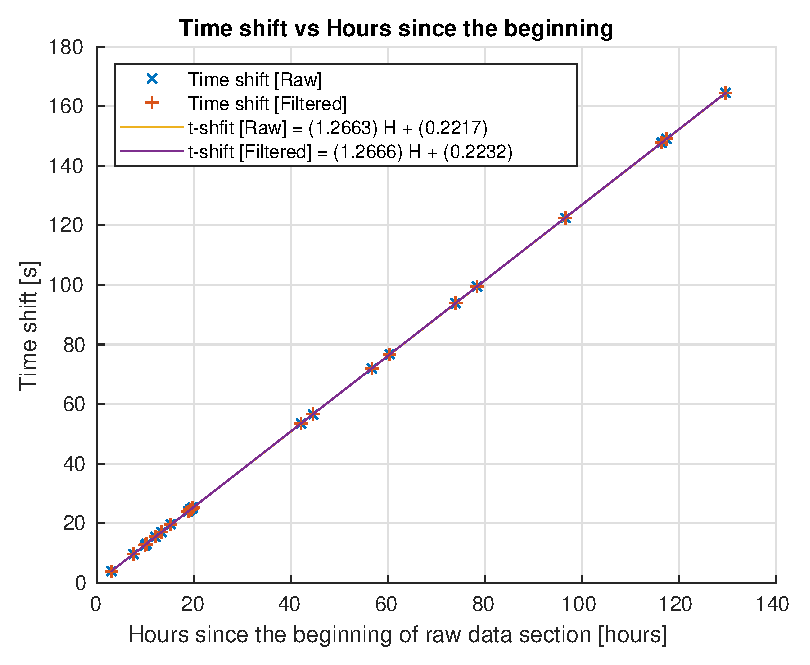
\includegraphics[width=0.7\linewidth]{Figures/Plots/timeshift_vs_hours_since_beginning.eps}
    \caption{A plot of time shift versus hours since the beginning of raw data section. The linear trend fit the data well. The fitted lines for raw and filtered seismograms do not differ.}
    \label{fig:timeshift_vs_hours}
\end{figure}

\begin{figure}
    \centering
    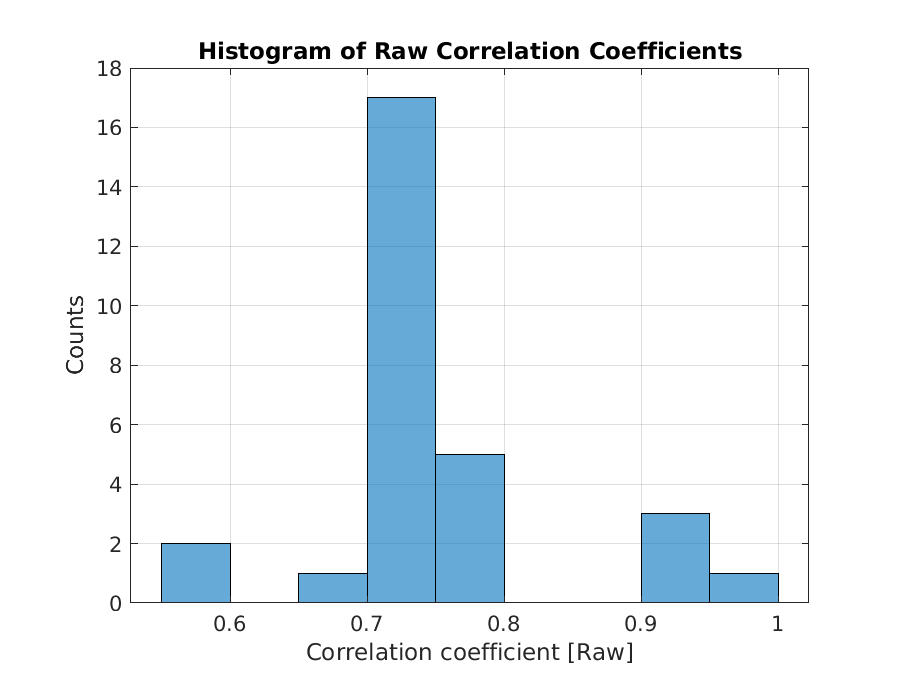
\includegraphics[width=0.7\linewidth]{Figures/Plots/raw_cc_histogram.eps}
    \caption{Caption}
    \label{fig:raw_cc_histogram}
\end{figure}

\begin{figure}
    \centering
    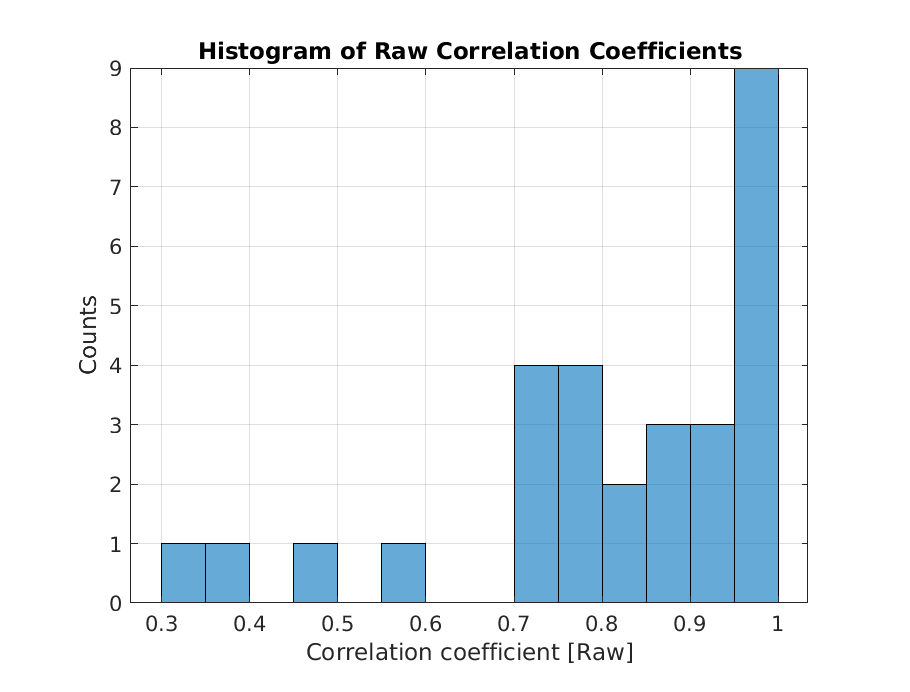
\includegraphics[width=0.7\linewidth]{Figures/Plots/filtered_cc_histogram.eps}
    \caption{Caption}
    \label{fig:filtered_cc_histogram}
\end{figure}

\begin{figure}
    \centering
    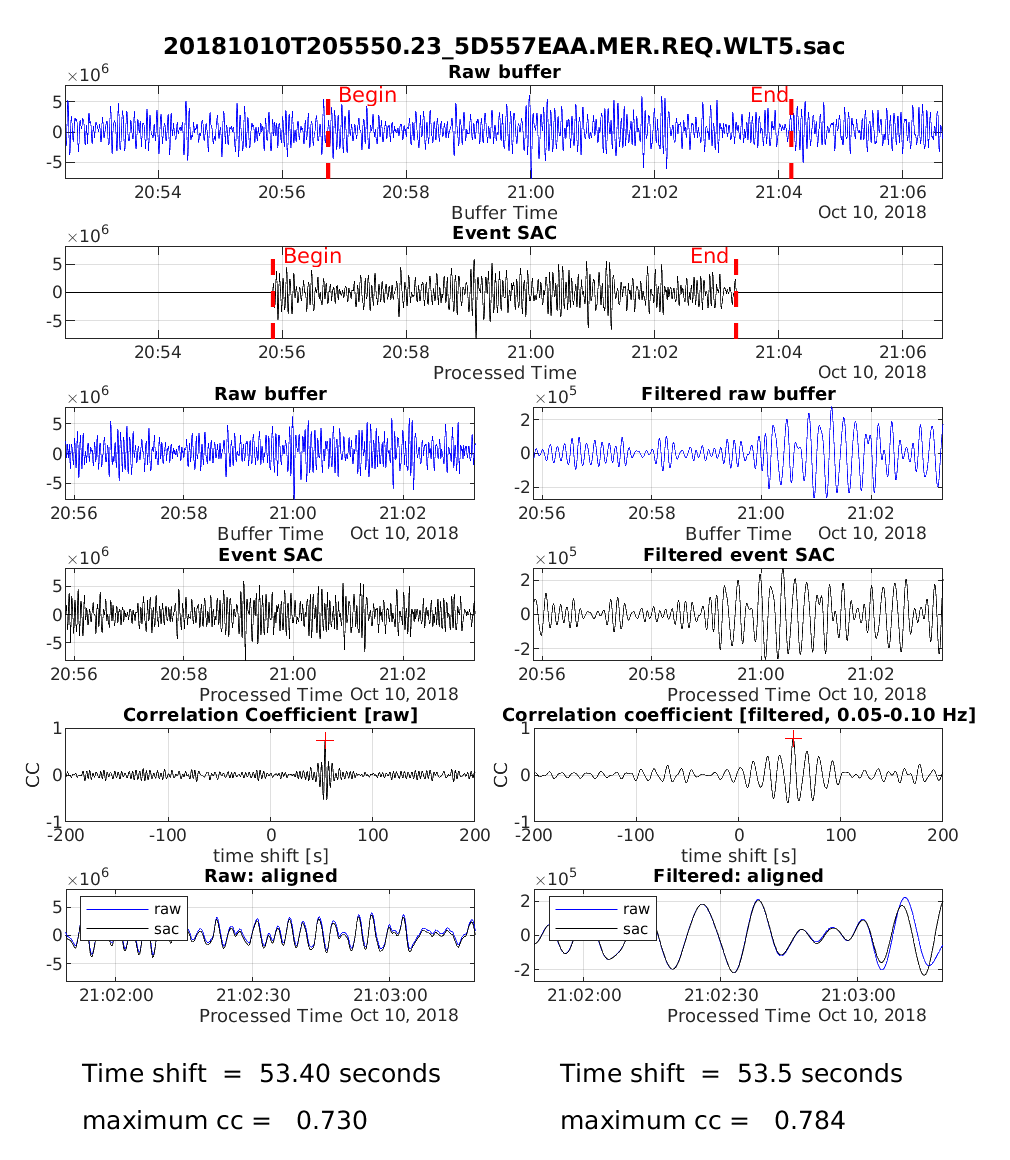
\includegraphics[width=\linewidth]{Figures/Matched_SACs/20181010T205550.eps}
    \caption{Caption}
    \label{fig:matched_01}
\end{figure}

\begin{figure}
    \centering
    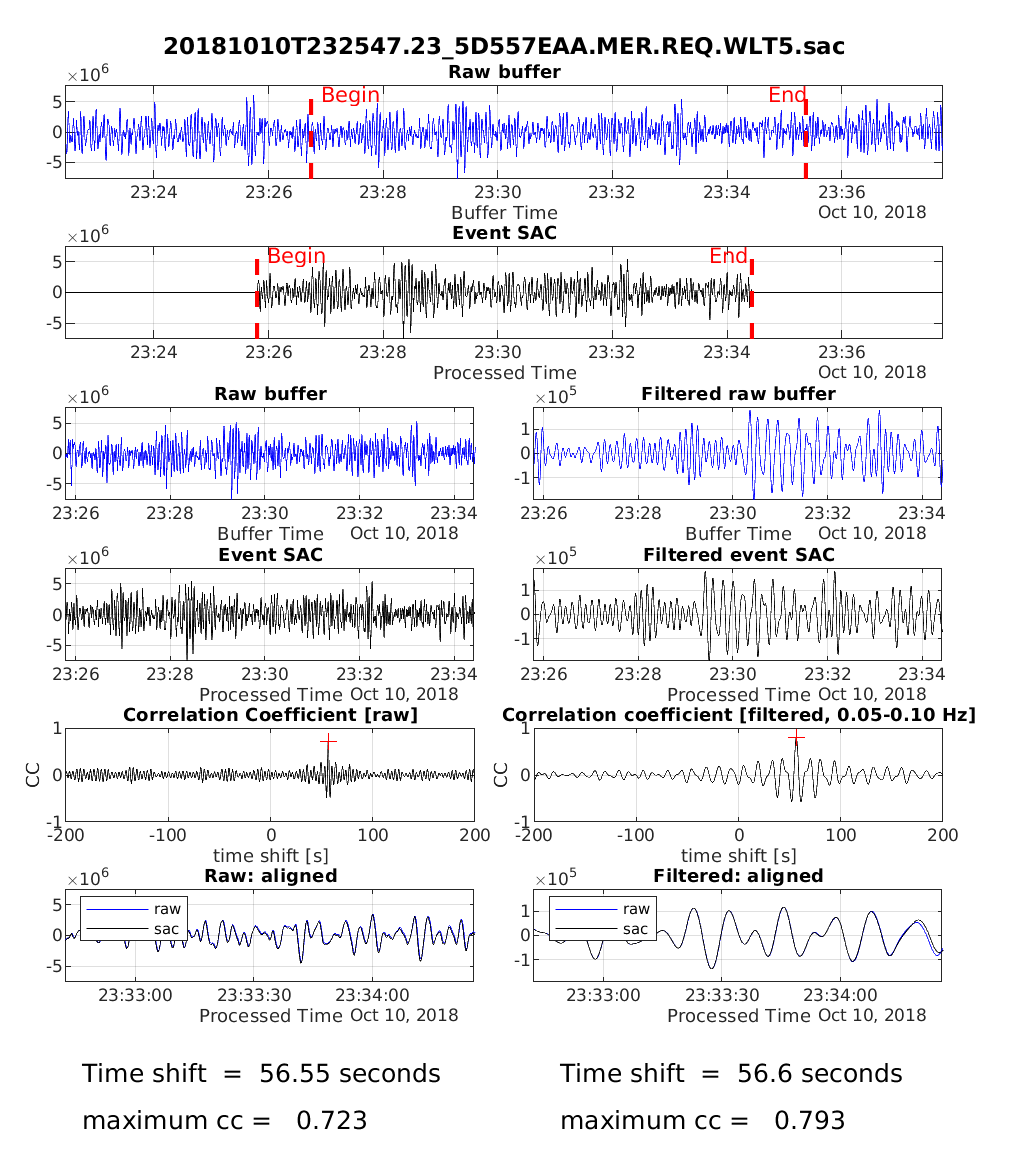
\includegraphics[width=\linewidth]{Figures/Matched_SACs/20181010T232547.eps}
    \caption{Caption}
    \label{fig:matched_02}
\end{figure}

\begin{figure}
    \centering
    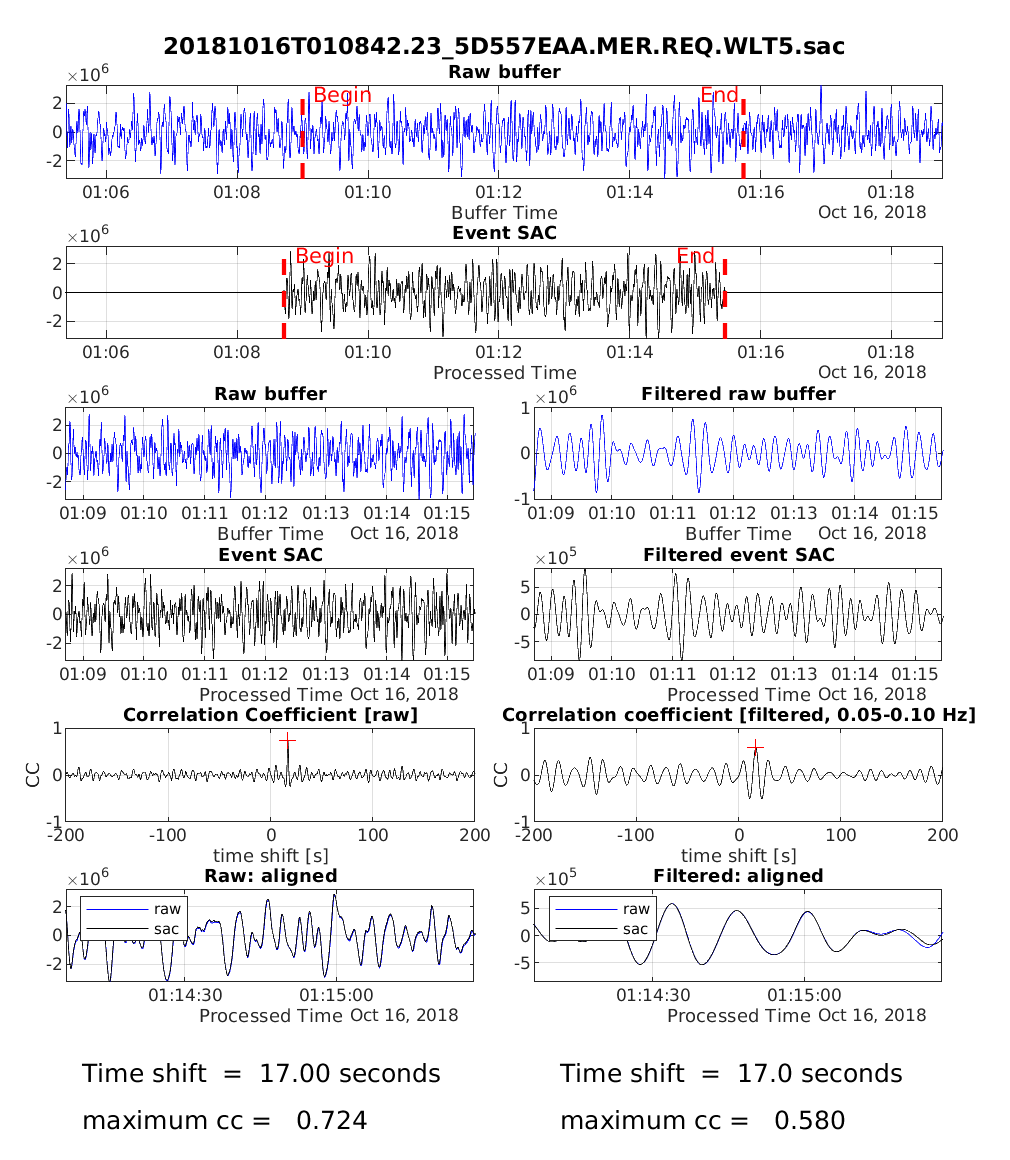
\includegraphics[width=\linewidth]{Figures/Matched_SACs/20181016T010842.eps}
    \caption{Caption}
    \label{fig:matched_03}
\end{figure}

\begin{figure}
    \centering
    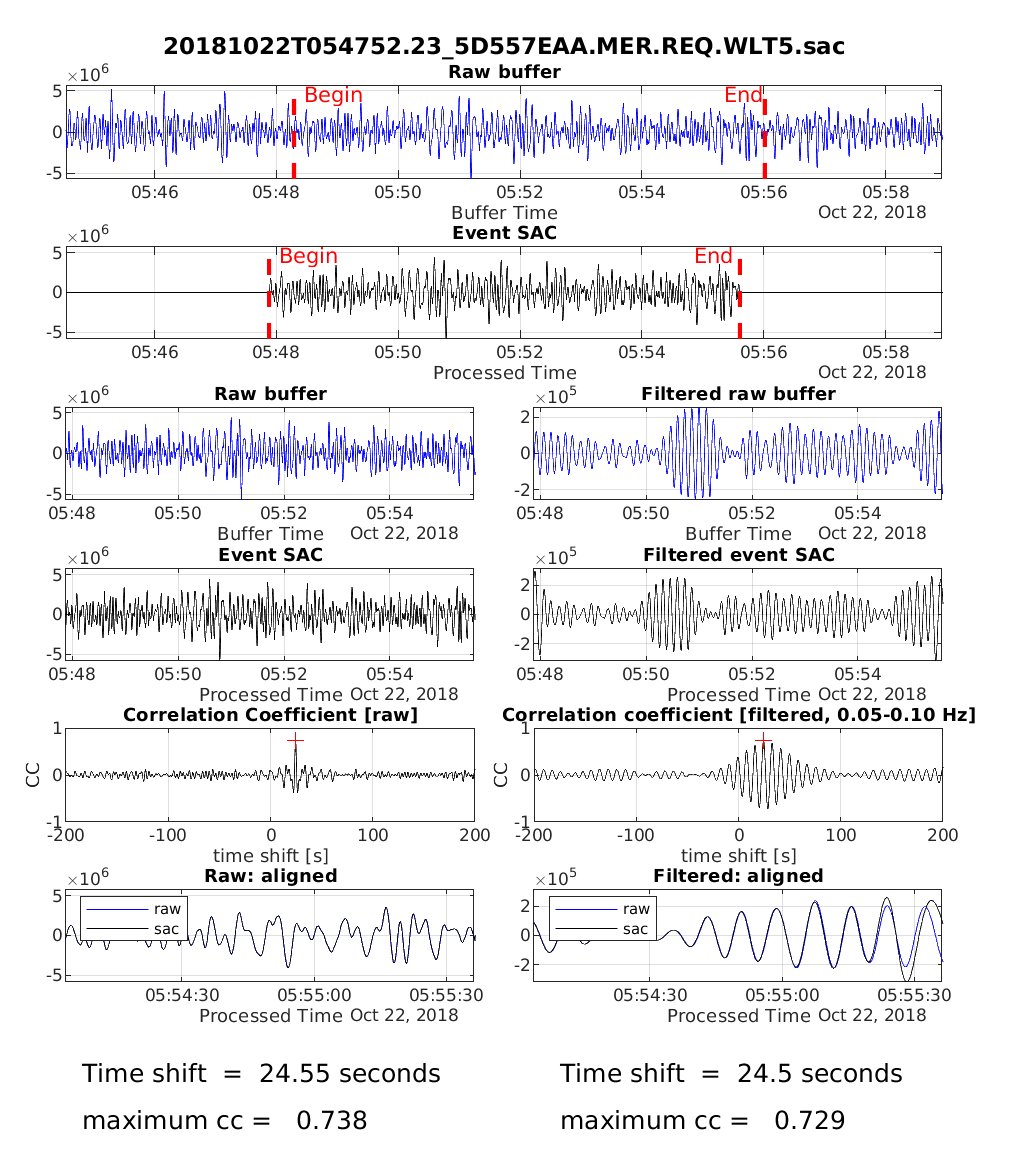
\includegraphics[width=\linewidth]{Figures/Matched_SACs/20181022T054752.eps}
    \caption{Caption}
    \label{fig:matched_04}
\end{figure}

\begin{figure}
    \centering
    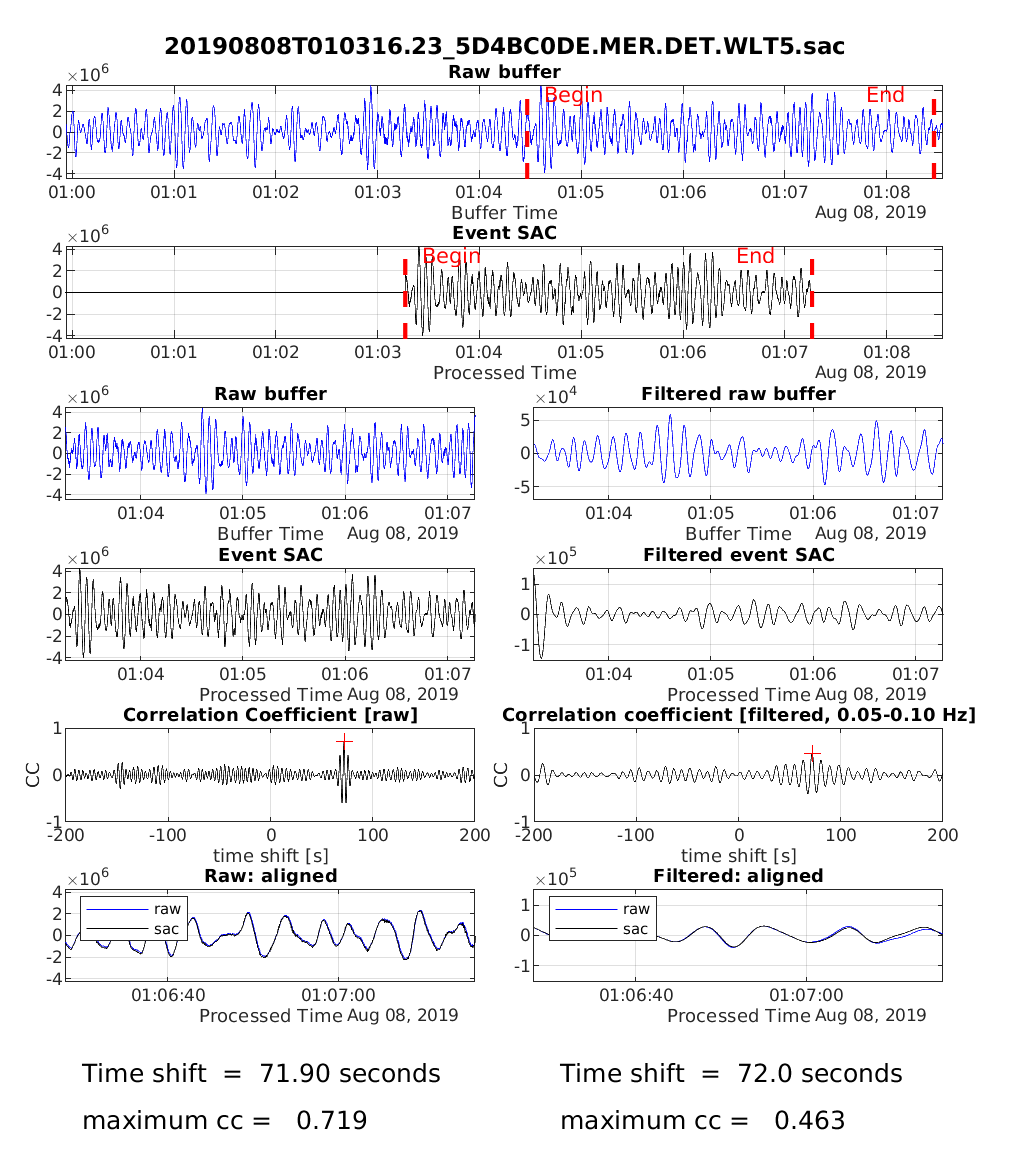
\includegraphics[width=\linewidth]{Figures/Matched_SACs/20190808T010316.eps}
    \caption{Caption}
    \label{fig:matched_end}
\end{figure}
\end{document}
